\documentclass[a4paper,12pt]{article}
\usepackage{graphicx}
\usepackage{amsmath, amssymb}
\usepackage{geometry}
\usepackage{hyperref}
\usepackage{tikz}
\usetikzlibrary{shapes.geometric, arrows}
\usepackage{float}
\geometry{margin=1in}
\title{Factory Alcohol Detection System}
\author{Bayanda Dlamini}
\date{\today}
\begin{document}
\maketitle
\section{Introduction}
This report details the design of a Factory Alcohol Detection System to prevent intoxicated employees from entering the workplace, ensuring compliance with the Occupational Safety and Health Act, 2001 (No. 9 of 2001) of Eswatini. The system integrates alcohol detection with controlled access and incident logging to enhance workplace safety.

\section{System Overview}
\subsection{Operational Flow}
\begin{enumerate}
    \item Employee enters the mantrap.
    \item System verifies identity using fingerprint scanning.
    \item Alcohol sensor analyzes breath.
    \item If within limits, exit opens; otherwise, alarm triggers, details are logged, and prior records are checked for suspension/dismissal.
\end{enumerate}

\section{Study of the Plant (Factory Entrance and Access Control)}
\subsection{Purpose and Operation}
The system regulates employee access via a mantrap, preventing intoxicated individuals from entering. It verifies identity using fingerprint scanning, analyzes breath samples, and grants or denies access based on alcohol levels.

\subsection{Inputs and Outputs}
\begin{itemize}
    \item Inputs: Breath alcohol concentration (BrAC), employee fingerprint data, environmental conditions.
    \item Outputs: Gate control, alarm activation, incident logs.
\end{itemize}

\begin{figure}[H]
    \centering
    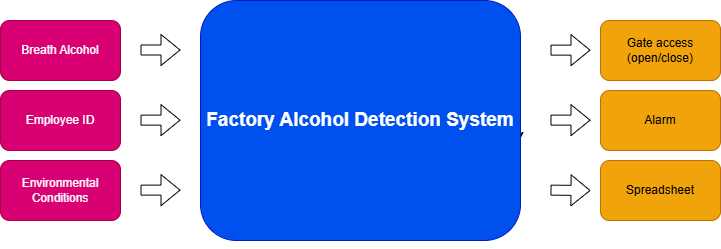
\includegraphics[width=0.8\textwidth]{images/flowChart.png}
    \caption{Block Diagram of Inputs and Outputs}
\end{figure}

\subsection{Relevant Variables}
\begin{itemize}
    \item State: BrAC, baseline alcohol, ID status.
    \item Operational: Employee flow, system response time.
\end{itemize}

\subsection{Challenges}
High traffic, environmental factors, and false positives.

\section{Subsystem Decomposition}
\subsection{Mechanical}
Mantrap structure, gate mechanism, testing chamber.

\begin{figure}[H]
    \centering
    \includegraphics[width=0.5\textwidth]{images/SecurityPortal.png}
    \caption{Image of Mantrap}
\end{figure}

\subsubsection{Physical Equations}
\begin{equation}
    F = m \cdot a
\end{equation}

\subsection{Electrical/Electronic}
Alcohol sensor, fingerprint scanner, microcontroller/PLC, actuators.
\subsubsection{Physical Equations}
\begin{equation}
    V_{out} = V_{baseline} + S \cdot \text{BrAC}
\end{equation}
\begin{equation}
    P_{total} = P_{sensor} + P_{controller} + P_{actuator}
\end{equation}

\subsection{Software}
Data acquisition, decision logic, logging.
\subsubsection{Control Logic}
\begin{equation}
    \text{Access} = 
    \begin{cases}
    \text{Granted}, & \text{if BrAC} \leq \text{Threshold} \\
    \text{Denied}, & \text{if BrAC} > \text{Threshold}
    \end{cases}
\end{equation}

\section{Operating Requirements (Performance Specifications)}
\begin{itemize}
    \item Alcohol Detection: Range 0.00\%-0.20\% BAC, accuracy $\pm 0.01\%$, response $\leq 3$ seconds.
    \item Access Control: Gate operation within 2 seconds, false positives $< 1\%$, false negatives $< 0.5\%$.
    \item Data Logging: Logs within 1 second, stores 10,000+ records, generates real-time reports.
    \item Environmental: Operates $-10^\circ$C to $40^\circ$C, 10\%-90\% humidity, resistant to dust.
    \item Power: 24V DC, $\leq 50W$.
    \item Reliability: 99.9\% uptime, sensor calibration every 6 months.
    \item Safety: 85 dB alarm.
    \item User Interface: Intuitive breath sample and fingerprint provision.
\end{itemize}

\section{Constraints}
\begin{itemize}
    \item Size/Weight: Fit within existing entrances.
    \item Environment: $0^\circ$C to $40^\circ$C, 10\%-90\% humidity, dust resistant.
    \item Power: 24V DC, $\leq 50W$.
    \item Security: Tamper-proof storage, secure communication, secure fingerprint data handling.
    \item Maintenance: Minimal, calibration every 6 months.
    \item Compliance: Occupational Safety and Health Act, 2001 (Eswatini).
\end{itemize}

\section{Component Selection}
\begin{itemize}
    \item Sensors: MQ-3 gas sensor, fingerprint scanner.
    \item Actuators: 24V DC door locks, 85 dB buzzer, LEDs.
    \item Microcontroller: Arduino Uno (prototype), industrial PLC (deployment).
    \item Power: 24V DC regulator.
    \item Storage: SD card module.
\end{itemize}

\section{System Architecture}
Mechanical, electrical/electronic, and software subsystems, as described earlier.

\subsection{Flowchart}
\tikzstyle{startstop} = [rectangle, rounded corners, minimum width=3cm, minimum height=1cm,text centered, draw=black, fill=red!30]
\tikzstyle{process} = [rectangle, minimum width=3cm, minimum height=1cm, text centered, draw=black, fill=blue!20]
\tikzstyle{decision} = [diamond, minimum width=3cm, minimum height=1cm, text centered, draw=black, fill=yellow!30]
\tikzstyle{arrow} = [thick,->,>=stealth]
\begin{figure}[H]
    \centering
    \begin{tikzpicture}[node distance=2cm]
        \node (start) [startstop] {Start};
        \node (idCheck) [process, below of=start] {Employee scans Fingerprint};
        \node (baseline) [process, below of=idCheck] {Read baseline alcohol level};
        \node (test) [process, below of=baseline] {Employee provides breath sample};
        \node (analyze) [process, below of=test] {Analyze alcohol level};
        \node (decision) [decision, below of=analyze] {Above limit?};
        \node (suspendCheck) [decision, right of=decision, xshift=4cm] {Prior offense?};
        \node (suspend) [startstop, below of=suspendCheck, yshift=-2cm] {Suspend Employee, Log Incident};
        \node (deny) [startstop, above of=suspendCheck, yshift=2cm] {Access Denied, Log Incident};
        \node (allow) [startstop, below of=decision, yshift=-2cm] {Grant Access};
        
        \draw [arrow] (start) -- (idCheck);
        \draw [arrow] (idCheck) -- (baseline);
        \draw [arrow] (baseline) -- (test);
        \draw [arrow] (test) -- (analyze);
        \draw [arrow] (analyze) -- (decision);
        \draw [arrow] (decision.east) -- (suspendCheck.west) node[midway, above] {Yes};
        \draw [arrow] (suspendCheck.north) -- (deny.south) node[midway, right] {No Prior Offense};
        \draw [arrow] (suspendCheck.south) -- (suspend.north) node[midway, right] {Prior Offense};
        \draw [arrow] (decision.south) -- (allow.north) node[midway, right] {No};
    \end{tikzpicture}
    \caption{Flowchart of Alcohol Detection System}
\end{figure}

\section{Implementation Plan}
Phased approach: prototype, field testing, full deployment, monitoring/optimization.

\section{Conclusion}
The system enhances workplace safety via integrated alcohol detection and access control using fingerprint verification, complying with Eswatini's safety regulations. Future work: scalability and additional safety features.

\section{References}
\begin{itemize}
    \item Occupational Safety and Health Act, 2001 (No. 9 of 2001), Eswatini.
    \item EEE428 - Instrumentation Systems. (Course Materials).
\end{itemize}
\end{document}